\let\negmedspace\undefined
\let\negthickspace\undefined

\documentclass[journal,11pt,twocolumn]{IEEEtran}

\usepackage{gensymb}
\usepackage{polynom}
\usepackage{amssymb}
\usepackage[cmex10]{amsmath}
\usepackage{amsthm}
\usepackage{stfloats}
\usepackage{bm}
\usepackage{longtable}
\usepackage{enumitem}
\usepackage{mathtools}
\usepackage{tikz}
\usepackage[breaklinks=true]{hyperref}
\usepackage{listings}
    \usepackage{color}                                            %%
    \usepackage{array}                                            %%
    \usepackage{longtable}                                        %%
    \usepackage{calc}                                             %%
    \usepackage{multirow}                                         %%
    \usepackage{hhline}                                           %%
    \usepackage{ifthen}                                           %%
  
\usepackage{lscape}     
\usepackage{tfrupee}

\pagecolor{white}
\DeclareMathOperator*{\Res}{Res}
\DeclareMathOperator*{\equals}{=}

\hyphenation{op-tical net-works semi-conduc-tor}
\def\inputGnumericTable{}                                 %%


\graphicspath{{./images}}
\begin{document}

	\title{Assignment 2 : Question 15 (b)}
	\author{ Abhay Shankar K : cs21btech11001}

	\maketitle

	\bigskip

	\providecommand{\brak}[1]{\ensuremath{\left(#1\right)}}
	\providecommand{\abs}[1]{\left\vert#1\right\vert}
	\providecommand{\norm}[1]{\left\lVert#1\right\rVert}
	\newcommand{\solution}{\noindent \textbf{Solution: }}
	\newcommand{\question}{\noindent \textbf{Question: }}

	\newcommand{\myvec}[1]{\ensuremath{\begin{pmatrix}#1\end{pmatrix}}}
	\newcommand{\mydet}[1]{\ensuremath{\begin{vmatrix}#1\end{vmatrix}}}

	\makeatletter
	\@addtoreset{figure}{problem}
	\makeatother
	\let\StandardTheFigure\thefigure
	\let\vec\mathbf

	\question

	Find the length of the perpendicular from the origin to the plane
	\begin{align} \label{given}
		\vec{r} \cdot \brak{3i - 4j - 12k} + 39 = 0
	\end{align}

	\solution
	Clearly, the length of the perpendicular from a plane passing through some point is the distance of that point from the plane.

	The normal form of a plane is an equation of the form:
	\begin{align}\label{Gen_plane}
		\vec{A}\vec{x} = D
	\end{align}

	Where :
	\begin{itemize}
		\item $\vec{A} = \myvec{a & b & c}$
		\item $\vec{x} = \myvec{x \\ y \\ z}$, called the point vector
		\item D is some scalar constant.
	\end{itemize}

	We can represent the given plane \brak{equation ~\eqref{given}} using normal form from \brak{equation ~\eqref{Gen_plane}} thus :
	\begin{align}
        		\label{normal_form}
		\myvec{3 & -4 & -12} \vec{x} & = -39\\
		\intertext{The formula for the distance of a point from a plane is :}
		\label{4-vec}
		Distance & = \frac{1}{\norm{\vec{A}}}  \abs{\myvec{a & b & c & D} \cdot \myvec{x \\ y \\ z \\1}}
		\intertext{The input parameters for equation $~\eqref{4-vec}$ are:}
		\label{A_sub}
		\vec{A} &= \myvec{a & b & c} =  \myvec{3 & -4 & -12}\\
		\label{x_sub}
		\vec{x} &= \myvec{x \\ y \\ z} =  \myvec{0 \\ 0 \\ 0}\\
		\label{D_sub}
		D &= -39
		\intertext{Upon substitution of equations $ \eqref{A_sub}, ~\eqref{x_sub}, ~\eqref{D_sub}$ into equation $\eqref{4-vec}$, }
		Distance &= \frac{1}{\norm{\vec{A}}}  \abs{\myvec{a & b & c & D} \cdot \myvec{x \\ y \\ z \\1}}\\
 				&= \frac{\abs{\myvec{3 & -4 & -12 & -39} \cdot \myvec{0 \\ 0 \\ 0 \\1}}}{\sqrt{3^2 + \brak{-4}^2 + \brak{-12}^2}}  \\
 				&= \frac{\abs{-39}}{\sqrt{169}}\\
 				&= \underline{3} \text{ units}
	\end{align}

	$\therefore$ The length of the perpendicular from the origin to the plane \brak{equation ~\eqref{given}} is \underline{$3$} units.

	\begin{figure}[h!]
		\centering
		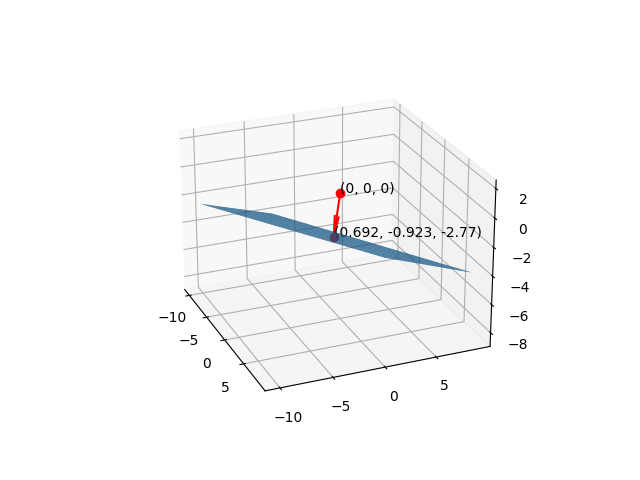
\includegraphics[width=\linewidth]{Graph_3D}
		\caption{Graph of the given plane}
	\end{figure}


\end{document}
